% =====================================================================
%  Using the Lunar-HFE Code — a developer & user guidebook
%  Self-contained for Overleaf: upload this folder (code_guide.tex +
%  figures/).  Compile with pdflatex (latexmk -pdf code_guide.tex).
% =====================================================================
\documentclass[11pt]{report}

\usepackage[a4paper,margin=2.4cm]{geometry}
\setlength{\emergencystretch}{3em}   % absorb unbreakable monospace paths
\usepackage[T1]{fontenc}
\usepackage{lmodern}
\usepackage[scaled=0.85]{beramono}   % readable monospace for listings
\usepackage{microtype}
\usepackage{amsmath,amssymb}
\usepackage{graphicx}
\usepackage{booktabs}
\usepackage{array}
\usepackage{xcolor}
\usepackage{listings}
\usepackage[most]{tcolorbox}
\usepackage{enumitem}
\usepackage{titlesec}
\usepackage[hidelinks]{hyperref}
\usepackage{fancyhdr}

% ---- palette (matches lunar/plotting/style.py) ----------------------
\definecolor{forest}{HTML}{3D6E4A}   % lunar/ (engine)
\definecolor{coral}{HTML}{B85B3A}    % scripts/
\definecolor{teal}{HTML}{2C6E73}     % paper/
\definecolor{char}{HTML}{2B2B2B}     % charcoal text
\definecolor{dim}{HTML}{6B6B6B}      % muted
\definecolor{paper}{HTML}{FBFAF7}
\definecolor{codebg}{HTML}{F4F2EE}
\definecolor{rulec}{HTML}{D8D2C8}

\hypersetup{linkcolor=teal,urlcolor=teal,citecolor=teal,
            colorlinks=true,allcolors=teal}

% ---- headings -------------------------------------------------------
\titleformat{\chapter}[display]
  {\normalfont\sffamily\bfseries\color{forest}}
  {\Large\color{dim}Chapter \thechapter}{4pt}{\Huge}
\titleformat{\section}{\normalfont\sffamily\large\bfseries\color{forest}}{\thesection}{0.7em}{}
\titleformat{\subsection}{\normalfont\sffamily\bfseries\color{char}}{\thesubsection}{0.6em}{}
\titlespacing*{\chapter}{0pt}{8pt}{18pt}

\pagestyle{fancy}\fancyhf{}
\renewcommand{\headrulewidth}{0.4pt}
\fancyhead[L]{\sffamily\small\color{dim}Using the Lunar-HFE Code}
\fancyhead[R]{\sffamily\small\color{dim}\thepage}

% ---- code listings --------------------------------------------------
\lstdefinestyle{py}{
  language=Python, basicstyle=\ttfamily\small\color{char},
  backgroundcolor=\color{codebg}, frame=single, framerule=0pt,
  rulecolor=\color{rulec}, keywordstyle=\color{forest}\bfseries,
  commentstyle=\color{dim}\itshape, stringstyle=\color{coral},
  showstringspaces=false, breaklines=true, columns=fullflexible,
  xleftmargin=8pt, xrightmargin=4pt, aboveskip=8pt, belowskip=8pt,
  literate={->}{{$\rightarrow$}}1 {>=}{{$\geq$}}1 {<=}{{$\leq$}}1,
}
\lstdefinestyle{sh}{
  language=bash, basicstyle=\ttfamily\small\color{char},
  backgroundcolor=\color{codebg}, frame=single, framerule=0pt,
  rulecolor=\color{rulec}, keywordstyle=\color{char},
  commentstyle=\color{forest}\itshape, showstringspaces=false,
  breaklines=true, columns=fullflexible, xleftmargin=8pt,
  morekeywords={make,python,python3,pip,git,jupyter,cd,source,pytest},
}
\newcommand{\code}[1]{{\ttfamily\small #1}}

% ---- callout boxes --------------------------------------------------
\newtcolorbox{plain}[1][]{colback=forest!6,colframe=forest!55,
  boxrule=0.6pt,arc=2pt,left=8pt,right=8pt,top=5pt,bottom=5pt,
  title={\sffamily\bfseries In plain words},coltitle=forest,fonttitle=\small,#1}
\newtcolorbox{tipbox}[1][]{colback=teal!6,colframe=teal!55,
  boxrule=0.6pt,arc=2pt,left=8pt,right=8pt,top=5pt,bottom=5pt,
  title={\sffamily\bfseries Tip},coltitle=teal,fonttitle=\small,#1}
\newtcolorbox{gotcha}[1][]{colback=coral!7,colframe=coral!60,
  boxrule=0.6pt,arc=2pt,left=8pt,right=8pt,top=5pt,bottom=5pt,
  title={\sffamily\bfseries Gotcha},coltitle=coral,fonttitle=\small,#1}

\newcommand{\file}[1]{\textcolor{forest}{\ttfamily #1}}
\setlist{leftmargin=1.4em,itemsep=2pt,topsep=3pt}

% =====================================================================
\begin{document}

\begin{titlepage}
\centering
\vspace*{3cm}
{\sffamily\bfseries\color{forest}\Huge Using the Lunar-HFE Code\par}
\vspace{8mm}
{\sffamily\Large\color{char} A developer \& user guidebook\par}
\vspace{4mm}
{\large\color{dim} How the package fits together, how to run it,\\
and how to change it without breaking anything\par}
\vfill
{\color{dim} Companion to the science guidebook (\file{paper/guidebook/guidebook.tex})\\
and the quick map (\file{docs/CODE\_MANUAL.md}). Repository:
\href{https://github.com/rp3gregorio/Lunar-HFE}{github.com/rp3gregorio/Lunar-HFE}\par}
\vspace{1cm}
{\color{dim} R.\,P.\ Gregorio \textperiodcentered\ Kasai Laboratory, Institute of Science Tokyo\par}
\end{titlepage}

\tableofcontents
\clearpage

% =====================================================================
\chapter{Orientation}
% =====================================================================

This guidebook teaches you the \emph{code}. If you want the physics and
statistics, read \file{paper/guidebook/guidebook.tex}; if you want a
one-page map, read \file{docs/CODE\_MANUAL.md}. Here we go deeper: every
module, every entry point, the exact function signatures, and a set of
worked recipes for the changes you are most likely to make.

\section{What the code does, in one sentence}

Given the Apollo~15 and~17 heat-flow temperature records, the code solves
a 1-D heat-conduction model of the regolith to a certified periodic
steady state, sweeps the deep thermal conductivity $K_d$ until the
modelled meter-scale temperatures best match the data, and quantifies the
uncertainty by bootstrap and Bayesian cross-check --- then draws every
figure and writes every number used in the paper.

\section{The mental model: three layers}

The single most useful thing to internalise is that the repository is
\textbf{layered}, and imports only ever point \textbf{downward}
(Figure~\ref{fig:arch}).

\begin{figure}[h]
\centering
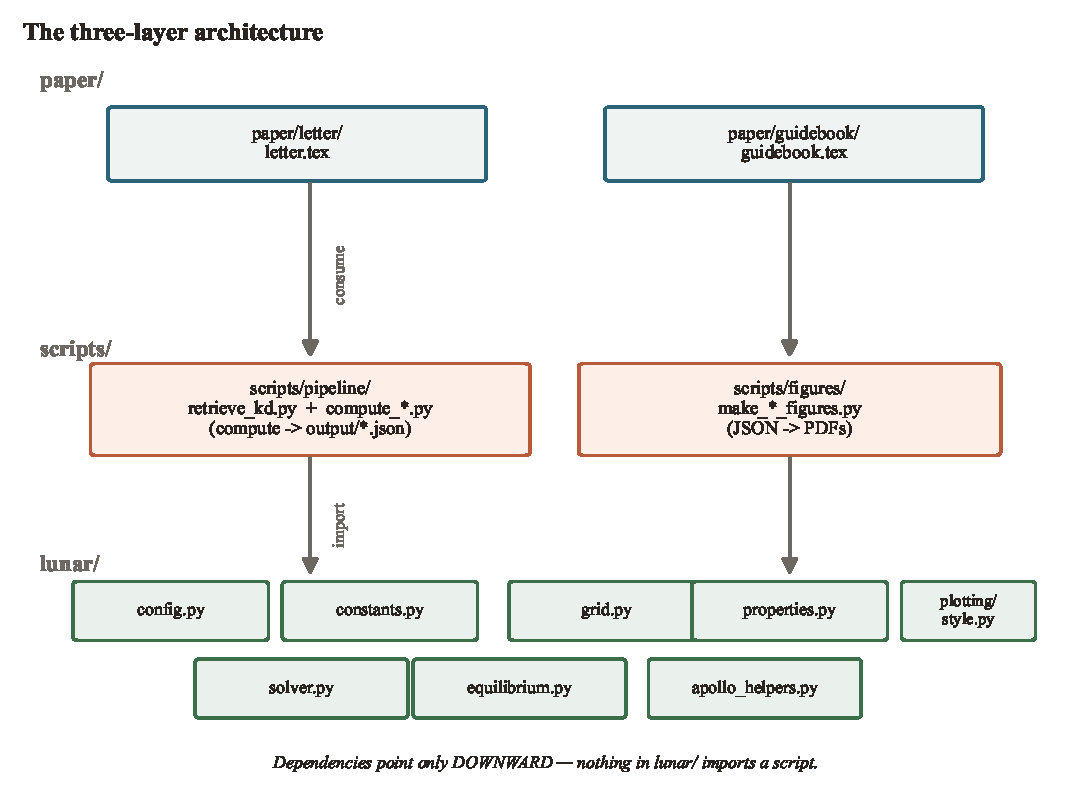
\includegraphics[width=\linewidth]{figures/fig_architecture.pdf}
\caption{The three layers. \file{lunar/} is the installable package (the
physics engine, the one configuration file, and the shared plotting
style). \file{scripts/} are thin command-line drivers that import the
package. \file{paper/} consumes the results. Nothing in \file{lunar/}
imports a script.}
\label{fig:arch}
\end{figure}

\begin{plain}
Think of \file{lunar/} as a \emph{library} you installed (like NumPy), and
\file{scripts/} as the little programs you wrote that \emph{use} that
library. You change behaviour by editing the library or its config; you
\emph{run} things by calling the scripts.
\end{plain}

\section{How a result travels}

Every number in the paper follows the same path
(Figure~\ref{fig:flow}): configuration $\rightarrow$ material models
$\rightarrow$ solver $\rightarrow$ \code{run\_with()} $\rightarrow$ sweep
\& bootstrap $\rightarrow$ a JSON file in \file{output/} $\rightarrow$ a
figure script $\rightarrow$ a PDF in \file{paper/}.

\begin{figure}[h]
\centering
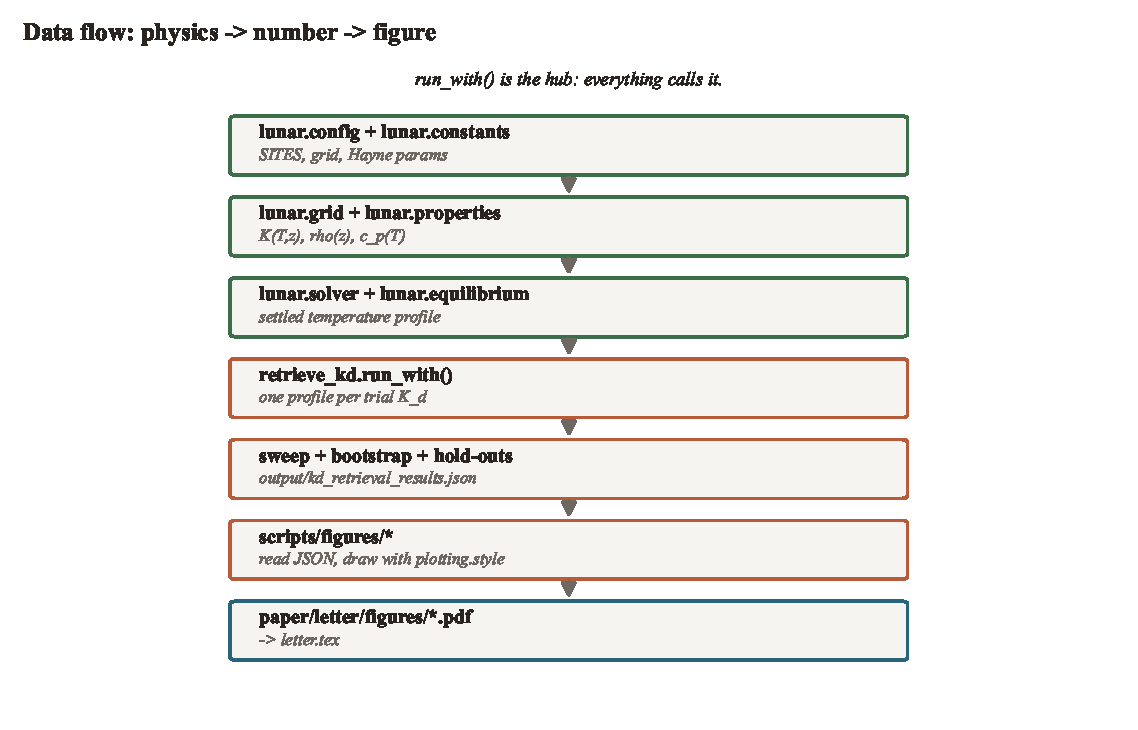
\includegraphics[width=0.92\linewidth]{figures/fig_dataflow.pdf}
\caption{The physics$\rightarrow$number$\rightarrow$figure pipeline. The
function \code{run\_with()} in \file{retrieve\_kd.py} is the hub: it turns
one trial $K_d$ into one settled temperature profile, and everything
above it (sweeps, bootstrap, sensitivities, figures) calls it.}
\label{fig:flow}
\end{figure}

\begin{tipbox}
If you remember only one function name, remember \code{run\_with()}. Once
you understand its inputs and its single output, you understand the whole
retrieval.
\end{tipbox}

% =====================================================================
\chapter{Setup and your first run}
% =====================================================================

\section{Prerequisites}
\begin{itemize}
\item Python $\geq 3.10$, a C compiler for NumPy/SciPy wheels (already
      present on macOS/Linux), and \code{git}.
\item A LaTeX distribution (TeX Live / MacTeX) only if you want to compile
      the PDFs; the science runs without it.
\item $\sim$\,1\,GB free disk if you fetch the Diviner cache (optional;
      only the surface-closure cross-check needs it).
\end{itemize}

\section{Install}

\begin{lstlisting}[style=sh]
git clone https://github.com/rp3gregorio/Lunar-HFE.git
cd Lunar-HFE
python3 -m venv .venv && source .venv/bin/activate
make install          # editable install of the lunar package + dev deps
\end{lstlisting}

\code{make install} runs \code{pip install -e .} so that \code{import
lunar} works from anywhere and your edits to \file{lunar/} take effect
immediately, with no reinstall.

\section{The one-word entry points}

Everything is driven by the \file{Makefile}. Run \code{make help} to list
targets; the important ones:

\begin{center}\small
\begin{tabular}{@{}lp{9.4cm}@{}}
\toprule
\code{make install} & editable install of \file{lunar/} + dev deps \\
\code{make retrieve} & core $K_d$ retrieval + bootstrap $\rightarrow$ \file{output/kd\_retrieval\_results.json} \\
\code{make aux} & every sensitivity sweep, model selection, MCMC, Diviner closure \\
\code{make figures} & regenerate every figure (calls \file{scripts/make\_all\_figures.py}) \\
\code{make paper} & compile the letter + guidebook PDFs \\
\code{make test} & the \code{pytest} suite (37 tests) \\
\code{make all} & \code{retrieve} $\rightarrow$ \code{aux} $\rightarrow$ \code{figures} $\rightarrow$ \code{paper} \\
\code{make clean} & remove LaTeX build artefacts \\
\bottomrule
\end{tabular}
\end{center}

\section{Your first run}

\begin{lstlisting}[style=sh]
make retrieve     # ~1-2 min: writes output/kd_retrieval_results.json
make test         # ~15 s: should report "37 passed"
make figures      # redraws the PDFs from the JSON you just made
\end{lstlisting}

After \code{make retrieve} you should see, near the end of the log, the
two headline numbers
\[
K_{d,\mathrm{A15}}^{*}\approx 4.6,\qquad
K_{d,\mathrm{A17}}^{*}\approx 8.1\ \ \mathrm{(mW\,m^{-1}\,K^{-1})},
\]
and the file \file{output/kd\_retrieval\_results.json} on disk. That file
is the canonical result; everything downstream reads it.

\begin{gotcha}
The Diviner surface-closure cross-check (\code{compute\_diviner\_closure})
needs the GCP cache, fetched once with \code{python
scripts/fetch\_diviner.py} ($\sim$310\,MB). If you skip it, that single
figure is skipped --- the retrieval itself does \emph{not} need Diviner.
\end{gotcha}

% =====================================================================
\chapter{The configuration: \texttt{lunar/config.py}}
% =====================================================================

This is the \textbf{single source of truth}. Almost every change you will
ever want starts here, and because every script reads these same objects,
a change propagates everywhere at once.

\section{The site table \texttt{SITES}}

A dictionary keyed \code{'A15'} / \code{'A17'}. Each entry carries the
physical description of one borehole:

\begin{center}\small
\begin{tabular}{@{}llp{7.6cm}@{}}
\toprule
Key & Example (A15) & Meaning \\
\midrule
\code{tag} & \code{'A15'} & short site label used in caches \\
\code{lat},\code{lon} & 26.13, 3.63 & landing-site coordinates [deg] \\
\code{albedo} & 0.131 & bolometric Bond albedo \\
\code{emissivity} & 0.95 & IR emissivity \\
\code{Q\_BASAL} & 0.021 & basal heat flux [W\,m$^{-2}$] (held fixed) \\
\code{T\_MEAN\_EFF} & 250.0 & seed mean temperature [K] (\emph{seed only}) \\
\code{MIN\_DEPTH\_CM} & 80 & borestem cut: ignore sensors above this \\
\code{mission} & \code{'a15'} & key into the bundled HFE data \\
\bottomrule
\end{tabular}
\end{center}

\begin{gotcha}
\code{T\_MEAN\_EFF} only \emph{seeds} the first iterate. The converged
profile is independent of it --- that guess-independence is exactly the
property the equilibrium solver guarantees (audit flag~F1). Do not treat
it as a tuning knob.
\end{gotcha}

\section{The other configuration objects}

\begin{center}\small
\begin{tabular}{@{}p{3.9cm}p{9.6cm}@{}}
\toprule
\code{GRID} & \code{dict(z\_max, dz0, growth)} --- depth mesh: max depth, top-layer thickness, geometric growth rate. \\
\code{HAYNE} & \code{dict(K\_S, H, CHI, T\_REF)} --- the Hayne (2017) $K(T,z)$ parameters. \\
\code{S0} & solar constant at 1\,AU [W\,m$^{-2}$]. \\
\code{T\_LUNAR} & one lunation [s]. \\
\code{DT\_STEP} & solver time step [s] (3600\,s = 1\,h). \\
\code{EQ\_Z\_ANCHOR, EQ\_N\_INNER, EQ\_MAX\_OUTER, EQ\_ANCHOR\_TOL} & equilibrium-solver controls (anchor depth, inner cycles, outer cap, convergence tol). \\
\code{KD\_GRIDS} & per-site array of trial $K_d$ values the sweep walks. \\
\code{DEPTH\_SIGMA\_CM} & sensor-depth jitter ($\pm$2.5\,cm) used by the bootstrap. \\
\code{TL\_*} & 3-layer-model parameters (reference depths, densities). \\
\bottomrule
\end{tabular}
\end{center}

\begin{tipbox}
\textbf{Worked change.} To test Apollo~15 with a 10\% higher basal flux,
edit one number:
\begin{lstlisting}[style=py]
SITES['A15']['Q_BASAL'] = 0.0231   # was 0.021
\end{lstlisting}
then \code{make retrieve}. The retrieval, every sensitivity script, and
every figure now use the new value --- no other file to touch.
\end{tipbox}

% =====================================================================
\chapter{The physics engine (\texttt{lunar/})}
% =====================================================================

These are the modules you import, not run. Signatures below are the real
ones in the code.

\section{\texttt{constants.py} --- cited numbers}

Every physical constant lives here with a source comment: the
Stefan--Boltzmann $\sigma$, the Hayne surface/deep conductivities
($K_S$, $K_d$), the $H$ and $\chi$ parameters, regolith densities, and the
specific-heat / Mart\'inez coefficients. \textbf{Never} hard-code a
constant in a script --- import it from here.

\section{\texttt{properties.py} --- material models}

\begin{lstlisting}[style=py]
conductivity_hayne(T, z, Ks=K_SURFACE, Kd=K_DEEP, H=..., chi=...)
conductivity_martinez(T, z=None, rho=None)
density_hayne(z, rho_s, rho_d, H)
specific_heat(T, model="hayne")        # or "biele"
\end{lstlisting}

\code{conductivity\_hayne} returns the temperature- and depth-dependent
conductivity $K(T,z)=K_c(z)\,[1+\chi(T/T_{\mathrm{ref}})^3]$ where the
solid term $K_c$ rises from $K_S$ at the surface to $K_d$ at depth. These
are pure functions of NumPy arrays --- no global state.

\section{\texttt{grid.py} --- the depth mesh}

\begin{lstlisting}[style=py]
g = make_geometric_grid(z_max=3.0, dz0=0.002, growth=0.15)
g.z_face   # cell-face depths [m], shape (N+1,), z_face[0] == 0
g.z_mid    # cell-centre depths [m], shape (N,)
g.dz       # cell thicknesses [m]
g.n_layers # number of cells
\end{lstlisting}

The grid is \emph{geometric}: thin at the top (millimetre cells to resolve
the diurnal skin depth) and growing with depth. Uniform grids are
forbidden by project rule --- they cannot resolve the skin and the meter
scale at once.

\section{\texttt{solver.py} --- one forward integration}

The low-level engine: \code{solve\_pixel(PixelInputs(...))} integrates the
Crank--Nicolson heat equation over the supplied forcing with a Newton
surface energy balance and a geothermal-flux bottom boundary, returning a
\code{PixelOutputs}. You rarely call this directly --- the equilibrium
solver wraps it.

\section{\texttt{equilibrium.py} --- the settled state (the F1 fix)}

This is the function that made the study correct. Its job: return the
\emph{periodic steady state}, independent of the initial guess.

\begin{lstlisting}[style=py]
solve_periodic_equilibrium(
    grid, t, insolation, albedo, emissivity, Q_b, K_func,
    cp_func=None, rho_func=None,
    T_guess=250.0, z_anchor=0.55,
    n_inner=12, max_outer=20, anchor_tol_K=0.005,
) -> EquilibriumResult
\end{lstlisting}

It alternates short skin-depth spin-ups with a mean-field reconstruction
that forces the cycle-mean flux to equal $Q_b$ at every depth, iterating
until the anchor temperature stops moving. The returned
\code{EquilibriumResult} carries both the answer and its certificate:

\begin{center}\small
\begin{tabular}{@{}lp{9.6cm}@{}}
\toprule
\code{out} & the final periodic cycle (\code{PixelOutputs}) \\
\code{T\_mean} & cycle-mean temperature profile [K] --- the science output \\
\code{n\_outer} & outer iterations used \\
\code{anchor\_K} & final anchor temperature $\langle T\rangle(z_0)$ [K] \\
\code{anchor\_drift\_K} & last inter-iteration change (convergence proof) \\
\code{flux\_closure} & $\max|\langle q\rangle-Q_b|/Q_b$ below the anchor \\
\code{converged} & boolean \\
\bottomrule
\end{tabular}
\end{center}

\begin{plain}
``Periodic steady state'' means: run the model long enough that each
lunation looks like the last one, and deep down the heat flowing through
matches the geothermal flux. \code{anchor\_drift\_K} and
\code{flux\_closure} are the two numbers that \emph{prove} you got there.
\end{plain}

\section{A minimal forward run by hand}

You can drive the engine yourself without any of the retrieval machinery:

\begin{lstlisting}[style=py]
import numpy as np
from lunar.config import SITES, GRID, HAYNE, S0, T_LUNAR, DT_STEP
from lunar.grid import make_geometric_grid
from lunar.properties import conductivity_hayne, specific_heat
from lunar.equilibrium import solve_periodic_equilibrium

site = SITES['A15']
g = make_geometric_grid(**GRID)
t = np.arange(0, T_LUNAR, DT_STEP)
cosz = np.clip(np.cos(2*np.pi*t/T_LUNAR), 0, None)   # toy forcing
insol = S0 * (1 - site['albedo']) * cosz

def K(T, z):
    return conductivity_hayne(T, z, Ks=HAYNE['K_S'],
                              Kd=4.6e-3, H=HAYNE['H'],
                              chi=HAYNE['CHI'])
eq = solve_periodic_equilibrium(
        grid=g, t=t, insolation=insol,
        albedo=site['albedo'], emissivity=site['emissivity'],
        Q_b=site['Q_BASAL'], K_func=K,
        cp_func=lambda T: specific_heat(T, model='hayne'),
        T_guess=site['T_MEAN_EFF'])
print(eq.converged, eq.anchor_drift_K, eq.T_mean[-1])
\end{lstlisting}

% =====================================================================
\chapter{The retrieval pipeline (\texttt{scripts/pipeline/})}
% =====================================================================

\section{\texttt{run\_with()} --- the hub}

\begin{lstlisting}[style=py]
run_with(site_cfg, *, kd=None, h=None, qb=None,
         k_model='hayne', rho_deep=None, martinez_alpha=None)
    -> (z_mid, T_mean)
\end{lstlisting}

Give it a site config and a trial $K_d$; it builds the grid and the
forcing, assembles the chosen conductivity model
(\code{'hayne'}, \code{'3layer'} or \code{'martinez'}), calls
\code{solve\_periodic\_equilibrium}, caches the result, and returns the
mid-cell depths and the settled mean profile. Results are memoised, so
repeated calls with the same arguments are free.

\begin{center}\small
\begin{tabular}{@{}lp{9.8cm}@{}}
\toprule
\code{kd} & deep conductivity [W\,m$^{-1}$\,K$^{-1}$]; required for \code{hayne}/\code{3layer} \\
\code{h} & override the Hayne $H$ depth scale (else config) \\
\code{qb} & override the basal flux (else \code{site['Q\_BASAL']}) \\
\code{k\_model} & \code{'hayne'} (default), \code{'3layer'}, or \code{'martinez'} \\
\code{rho\_deep} & deep bulk density override (3-layer model) \\
\code{martinez\_alpha} & density scalar for the Mart\'inez per-site retrieval \\
\bottomrule
\end{tabular}
\end{center}

\section{From profile to $K_d^{*}$}

\code{run\_with} is called once per trial $K_d$ to build a residual matrix
$R$ (modelled $-$ observed at each deep sensor). Then:

\begin{lstlisting}[style=py]
kd_star, rmse_star = kd_star_from_residuals(R, kd_grid)
\end{lstlisting}

fits a parabola to the RMSE-vs-$K_d$ curve and returns the sub-grid
minimum. Re-sampling sensors (with the $\pm2.5$\,cm depth jitter) and
repeating $N_{\mathrm{boot}}=1500$ times gives the bootstrap confidence
interval. The hold-out checks (train on one sensor set, predict the other;
leave-one-deepest-out) reuse the same residuals.

\section{What \texttt{retrieve\_kd.py} writes}

Running it (\code{make retrieve}) produces
\file{output/kd\_retrieval\_results.json} plus the bootstrap, robustness
and hold-out figures. That JSON is the spine of the paper.

\section{The \texttt{compute\_*} sensitivity scripts}

Each is a thin driver that imports \code{run\_with} /
\code{kd\_star\_from\_residuals} from \file{retrieve\_kd.py} and writes one
JSON. Because they all import the engine through \file{retrieve\_kd.py}
(which re-exports the single \code{lunar.config.SITES}), they cannot drift
out of sync with the main retrieval.

\begin{center}\small
\begin{tabular}{@{}ll@{}}
\toprule
Script & Writes \\
\midrule
\code{compute\_headline\_rmse.py} & \code{headline\_rmse.json} \\
\code{compute\_borestem\_sensitivity.py} & \code{borestem\_sensitivity.json} \\
\code{compute\_stability\_threshold\_sensitivity.py} & \code{stability\_threshold\_sensitivity.json} \\
\code{compute\_surface\_bias\_test.py} & \code{surface\_bias\_test.json} \\
\code{compute\_uniform\_kd\_sensitivity.py} & \code{uniform\_kd\_test.json} \\
\code{compute\_fixed\_input\_sensitivities.py} & \code{fixed\_input\_sensitivities.json} \\
\code{compute\_model\_selection.py} & \code{model\_selection.json} (AICc M1/M2/M3) \\
\code{compute\_error\_budget.py} & \code{kd\_error\_budget.json} (reads the above) \\
\code{bayesian\_crosscheck.py} & \code{bayesian\_crosscheck\_samples.json} + posterior figs \\
\code{compute\_diviner\_closure.py} & \code{diviner\_closure.json} + closure fig \\
\bottomrule
\end{tabular}
\end{center}

\code{make aux} runs all of them in the right order (\code{error\_budget}
last, since it consumes the others).

% =====================================================================
\chapter{The results: \texttt{output/*.json}}
% =====================================================================

The JSON files are the contract between the pipeline and the figures: the
pipeline writes them, the figure scripts and the paper read them. The
canonical one, \file{kd\_retrieval\_results.json}, contains for each site:

\begin{itemize}
\item \code{kd\_star}, \code{rmse\_star} --- the retrieved conductivity and its RMSE;
\item \code{kd\_grid}, \code{rmse\_curve} --- the full sweep (for the $K_d$-sweep figure);
\item \code{bootstrap} --- \code{median}, \code{ci\_lo}, \code{ci\_hi}, and the raw \code{samples};
\item \code{holdout}, \code{loo\_deepest} --- the cross-prediction diagnostics;
\item provenance (git hash, timestamp, config echo) so a figure can never be drawn from stale numbers silently.
\end{itemize}

\begin{tipbox}
To read a number out without any code:
\begin{lstlisting}[style=sh]
python -c "import json;d=json.load(open('output/kd_retrieval_results.json'));print(d['A17']['kd_star'])"
\end{lstlisting}
\end{tipbox}

% =====================================================================
\chapter{The figures (\texttt{scripts/figures/})}
% =====================================================================

Figure scripts \emph{read} \file{output/*.json} and \emph{draw} with the
shared style; they never recompute science. Every one imports
\code{lunar.plotting.style} (palette + \code{rcParams}) and
\code{lunar.config} (for \code{SITES}); the few that need a forward curve
import \code{run\_with}.

\begin{center}\small
\begin{tabular}{@{}ll@{}}
\toprule
Script & Produces \\
\midrule
\code{make\_intro\_figures.py} & probe schematic \\
\code{make\_context\_map\_figure.py} & landing-site map \\
\code{make\_apollo\_timeline.py} & stability-window timeline \\
\code{make\_letter\_figures.py} & amplitude, mean-$T$, $K_d$ sweep \\
\code{make\_results\_figures.py} & bootstrap + robustness panels \\
\code{make\_alpha\_sweep\_figure.py} & Mart\'inez $\alpha$-sweep \\
\code{make\_book\_figures.py}, \code{make\_primer\_figures.py} & guidebook teaching figures \\
\code{make\_equilibrium\_certification.py} & solver certification (to \file{output/figures/}) \\
\code{make\_codeguide\_figures.py} & the two diagrams in \emph{this} manual \\
\bottomrule
\end{tabular}
\end{center}

\code{scripts/make\_all\_figures.py} (\code{make figures}) runs them all,
timing each and reporting failures without stopping.

\section{The shared style}

\file{lunar/plotting/style.py} exports the palette
(\code{C\_A15}, \code{C\_A17}, \code{C\_HAYNE}, \dots), figure-width
constants, and helpers \code{fmt\_axis}, \code{legend\_below},
\code{legend\_outside}. Use them so every figure matches:

\begin{lstlisting}[style=py]
from lunar.plotting.style import C_A15, C_A17, fmt_axis, legend_below
fig, ax = plt.subplots()
ax.plot(x, y, color=C_A15, label="Apollo 15")
fmt_axis(ax, xlabel="depth [m]", ylabel="T [K]")
legend_below(ax)
\end{lstlisting}

\begin{gotcha}
Site \emph{presentation} colours live in the style module, not in
\code{config.SITES}. The config holds only physics. When a figure needs a
per-site colour, map it: \code{SITE\_COLOR = \{"A15": C\_A15, "A17":
C\_A17\}}.
\end{gotcha}

% =====================================================================
\chapter{Recipes}
% =====================================================================

\subsection*{Change a site parameter}
Edit the one number in \code{SITES} (Chapter~3) and \code{make retrieve}.

\subsection*{Retrieve under the Mart\'inez model instead of Hayne}
Call \code{run\_with(site, k\_model='martinez', martinez\_alpha=a)} in a
sweep over \code{a}; this is exactly what \code{make\_alpha\_sweep\_figure}
does. No engine change needed.

\subsection*{Run a single site interactively}
\begin{lstlisting}[style=py]
import sys; sys.path.insert(0, "scripts/pipeline")
from retrieve_kd import run_with
from lunar.config import SITES
z, T = run_with(SITES['A17'], kd=8.1e-3)
\end{lstlisting}

\subsection*{Regenerate just one figure}
\begin{lstlisting}[style=sh]
python -c "import sys;sys.path.insert(0,'scripts/figures');import make_letter_figures as m;m.main()"
\end{lstlisting}

\subsection*{Add a new site}
Add an entry to \code{SITES} with the eight fields, add a
\code{KD\_GRIDS['NEW']} array, ensure the bundled HFE data has the matching
\code{mission} key, and the entire pipeline picks it up. Add a colour in
\file{plotting/style.py} if you will plot it.

\subsection*{Add a new conductivity model}
Write the pure function in \file{properties.py}, register a branch for it
in \code{run\_with}'s \code{k\_model} dispatch, and it becomes available to
every sweep and figure.

\subsection*{Add a new sensitivity test}
Copy the smallest \code{compute\_*.py}, import \code{run\_with} /
\code{kd\_star\_from\_residuals}, write your JSON, and add a line to
\file{Makefile}'s \code{aux} target.

% =====================================================================
\chapter{Testing and reproducibility}
% =====================================================================

\code{make test} runs the \code{pytest} suite (37 tests): grid
monotonicity and skin resolution, conductivity/density model values
against cited numbers, solver energy conservation and the analytic
thermal-wave check, equilibrium guess-independence (start from two
different \code{T\_guess} values and assert the same converged profile),
and JSON-schema checks on the committed results.

\begin{itemize}
\item \textbf{Determinism:} the bootstrap and MCMC seed their RNGs, so
      reruns reproduce the published intervals bit-for-bit.
\item \textbf{Provenance:} each JSON records the git hash and config it was
      made with; a figure drawn from a stale file is detectable.
\item \textbf{Audit trail:} \file{docs/FLAG\_REPORT.md} lists every issue
      found in review (F1--F6) and how it was resolved.
\item \textbf{Notebooks:} the five \file{notebooks/} walk the same
      pipeline interactively and are a good place to learn by stepping.
\end{itemize}

% =====================================================================
\chapter{Toward the C++ port}
% =====================================================================

The Python layout is deliberately a clean reference for a faster C++
core. The numerics are isolated in three small, dependency-light modules
--- \file{grid.py}, \file{solver.py}, \file{equilibrium.py} --- with no
plotting or file I/O mixed in, all fed by a single \file{config.py}.

\begin{enumerate}
\item Port \file{grid.py} (pure array construction) first --- trivial and
      fully testable against the Python output.
\item Port \file{solver.py} (Crank--Nicolson + Thomas solve + Newton
      surface balance). Validate against the analytic thermal wave the
      Python test already uses.
\item Port \file{equilibrium.py} (the outer flux-anchored iteration).
\item Keep \file{config.py} as the single parameter file the C++ side
      \emph{also} reads (emit it as JSON), so there is still one source of
      truth.
\item Leave the analysis (\file{scripts/pipeline/}) and all figures in
      Python, calling the fast core through a thin binding.
\end{enumerate}

\begin{tipbox}
Port bottom-up and test each layer against the Python reference before
moving up. The 37-test suite is your regression harness across languages.
\end{tipbox}

% =====================================================================
\appendix
\chapter{Command cheat-sheet}
% =====================================================================

\begin{lstlisting}[style=sh]
make install     # editable install
make retrieve    # core retrieval + bootstrap  -> output/kd_retrieval_results.json
make aux         # all sensitivity sweeps + MCMC + closure
make figures     # redraw every figure
make paper       # compile the PDFs
make test        # pytest (37 tests)
make all         # everything, from scratch
make clean       # remove LaTeX build artefacts

# standalone equivalents
python scripts/pipeline/retrieve_kd.py
python scripts/make_all_figures.py
python scripts/figures/make_codeguide_figures.py   # this manual's diagrams
pytest -q
\end{lstlisting}

\chapter{Glossary of key objects}

\begin{center}\small
\begin{tabular}{@{}lp{9.8cm}@{}}
\toprule
\code{SITES} & the site table; one physics record per borehole \\
\code{make\_geometric\_grid} & builds the thin-at-top depth mesh (\code{DepthGrid}) \\
\code{conductivity\_hayne} & $K(T,z)$ used in the baseline retrieval \\
\code{solve\_periodic\_equilibrium} & the guess-independent settled-state solver \\
\code{EquilibriumResult} & the converged profile + its convergence certificate \\
\code{run\_with} & the hub: one trial $K_d$ $\rightarrow$ one settled profile \\
\code{kd\_star\_from\_residuals} & parabola-fit sub-grid minimum of the RMSE curve \\
\code{kd\_retrieval\_results.json} & the canonical result file everything downstream reads \\
\bottomrule
\end{tabular}
\end{center}

\vfill
\noindent\textcolor{dim}{\small Generated as a companion to the Lunar-HFE
repository. For the science behind the code, see
\file{paper/guidebook/guidebook.tex}.}

\end{document}
